\documentclass[border=10pt]{standalone}
\usepackage{pgfplots}
\pgfplotsset{compat=1.18}
\begin{document}
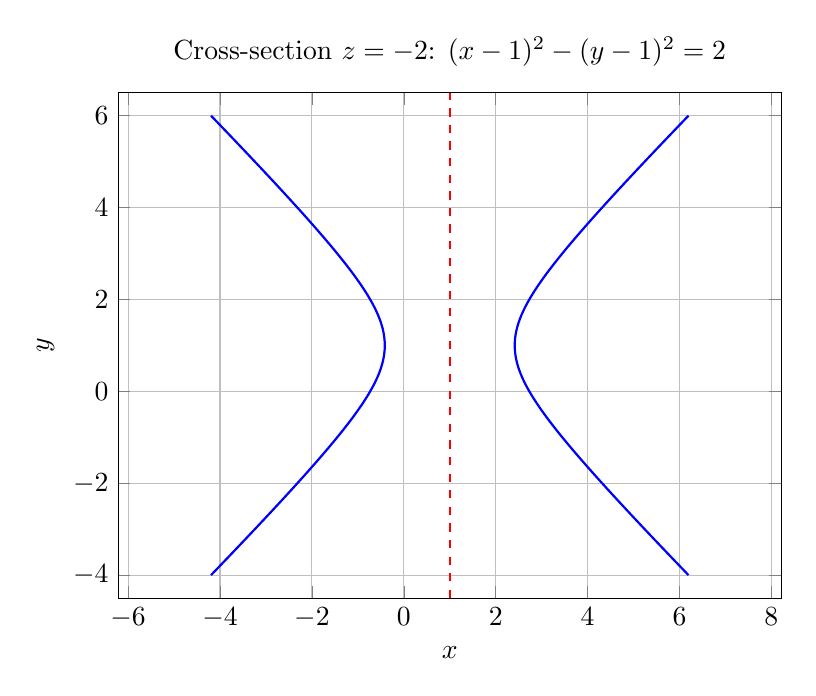
\begin{tikzpicture}
\begin{axis}[
  width=10cm, height=8cm,
  xlabel={$x$}, ylabel={$y$},
  title={Cross-section $z=-2$: $(x-1)^2-(y-1)^2=2$},
  grid=major,
  domain=-4:6,
  samples=200,
  axis equal,
  xmin=-4.5, xmax=6.5,
  ymin=-4.5, ymax=6.5
]
\addplot[blue, thick, domain=-4:6] ({1 + sqrt(2 + (x-1)^2)}, {x});
\addplot[blue, thick, domain=-4:6] ({1 - sqrt(2 + (x-1)^2)}, {x});
\addplot[red, dashed, thick] coordinates {(1,-4.5) (1,6.5)};
\end{axis}
\end{tikzpicture}
\end{document}